\documentclass{article}
\usepackage{graphics, latexsym}

\begin{document}

\newcommand{\SOPmin}{${\rm SOP}_{\rm min} \ $}
\newcommand{\POSmin}{${\rm POS}_{\rm min} \ $}
\newcommand{\bs}{\backslash}


\title{
\Huge{CSE 271 -- Fall 2004}\\
\normalsize{Return this exam!  No calculators!}\\
\normalsize{Exam 1}\\
\makebox[4in][l]{Name:}
SSN:}
\date{}

\maketitle{}

\begin{enumerate}
\item {\bf (2 pt.)} Convert $101101_2$ to decimal.
\begin{description}
\item{a) }42
\item{b) }45
\item{c) }49
\item{d) }84
\item{e) }None of the above.
\end{description}

\item {\bf (2 pt.)} Convert $73_{10}$ to binary.
\begin{description}
\item{a) }$1001001_2$
\item{b) }$1010111_2$
\item{c) }$0111111_2$
\item{d) }$1010010_2$
\item{e) }None of the above.
\end{description}

\item {\bf (2 pt.)} Convert $73_{16}$ to decimal.
\begin{description}
\item{a) }$115_{10}$
\item{b) }$71_{10}$
\item{c) }$57_{10}$
\item{d) }$39_{10}$
\item{e) }None of the above.
\end{description}
\pagebreak

\underline{For questions 4-7 assume $F(A,B,C)= (A(B'+C)' + A'B)'$ }

\item {\bf (2 pt.)} What does F(0,1,0) equal?
\begin{description}
\item{a) } 0
\item{b) } 1
\item{c) } B
\item{d) } B'
\item{e) } Not enough information.
\end{description}

\item {\bf (2 pt.)} What does F(1,B,1) equal?
\begin{description}
\item{a) } 0
\item{b) } 1
\item{c) } B
\item{d) } B'
\item{e) } Not enough information.
\end{description}

\item {\bf (2 pt.)} How many AND gates does it take to realize F 
as shown (do not simplify)?
\begin{description}
\item{a) } 1
\item{b) } 2
\item{c) } 3
\item{d) } 4
\item{e) } None of the above.
\end{description}


\item {\bf (2 pt.)} What is the \SOPmin expression for F?
\begin{description}
\item{a) } (A(B'+C)' + A'B)'
\item{b) } (ABC' + A'B)'
\item{c) } (A'+B'+C)(A + B')
\item{d) } A'B' + AB' + B' + AC + B'C
\item{e) } None of the above.
\end{description}

\pagebreak

\item {\bf (1 pt.)} Assume a word size of 6-bits.  If overflow occurs 
indicate it, otherwise identify the correct answer: $101010_2 + 011011_2$
\begin{description}
\item{a) }$000101_2$
\item{b) }$1000101_2$
\item{c) }$111111_2$
\item{d) }$101011_2$
\item{e) }Overflow occurs.
\end{description}

\vspace{0.2in}

\underline{For questions 9-10 use the figure below.}

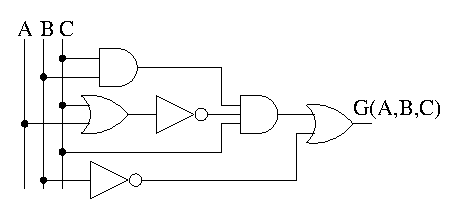
\includegraphics{./Fig1/cir_5}

\item {\bf (2 pt.)} What is the symbolic representation of $G(A,B,C)$ 
(do not simplify).
\begin{description}
\item{a) } BC + (A + C)' + B'
\item{b) } BC(A+C)' + B'
\item{c) } BC(A+C)'C + B'
\item{d) } B'
\item{e) } None of the above.
\end{description}

\item {\bf (2 pt.)} What is G(1,1,0)=?
\begin{description}
\item{a) } 1
\item{b) } 0
\end{description}

\item {\bf (2 pt.)} Does (X+Y)(X'+Z) = XZ + Y(X'+Z) ?
\begin{description}
\item{a) } Yes
\item{b) } No
\end{description}

\pagebreak

\item {\bf (2 pt.)} You are working on a kmap and find a legal grouping 
of 8 1's which requires 3 variables to represent.  How many variables 
does the function have?
\begin{description}
\item{a) } 3
\item{b) } 4
\item{c) } 5
\item{d) } 6
\item{e) } Not enough information.
\end{description}

\item {\bf (1 pt.)} A cell in a 7 variable kmap is adjacent to how many other cells?  
\begin{description}
\item{a) } 4
\item{b) } 6
\item{c) } 8
\item{d) } 10
\item{e) } None of the above.
\end{description}

\item {\bf (2 pt.)} How many rows does a truth table of 9 variables have?
\begin{description}
\item{a) } 81
\item{b) } 256
\item{c) } 512
\item{d) } 729
\item{e) } 1024
\end{description}


\item {\bf (1 pt.)} Which of the following is not shared by all the
representations of a logical function?
\begin{description}
\item{a) } a description of the number of inputs
\item{b) } a description of the number of outputs
\item{c) } a description of the circuits behavior
\item{d) } a descriptions of the circuits cost
\end{description}

\item {\bf (2 pt.)} How many different \SOPmin solutions exist for \\
F(A,B,C,D)=$\Sigma$m(0,1,3,6,7,8,10,12,13,15) ?
\marginpar{ \tiny $$ \begin{array} {c||c|c|c|c}
        AB \bs CD & 00 & 01 & 11 & 10 \\ \hline \hline
        00        &    &    &    &    \\ \hline
        01        &    &    &    &    \\ \hline
        11        &    &    &    &    \\ \hline
        10        &    &    &    &    \\ 
\end{array} $$ }
\begin{description}
\item{a) } 2
\item{b) } 4
\item{c) } 6
\item{d) } 12
\item{e) } None of the above
\end{description}

\pagebreak

\item {\bf (4 pt.)} Determine the \SOPmin expression for \\
F(A,B,C,D)=$\Sigma$m(1,2,3,7,8,10,15)
\marginpar{ \tiny $$ \begin{array} {c||c|c|c|c}
        AB \bs CD & 00 & 01 & 11 & 10 \\ \hline \hline
        00        &    &    &    &    \\ \hline
        01        &    &    &    &    \\ \hline
        11        &    &    &    &    \\ \hline
        10        &    &    &    &    \\
\end{array} $$ }
\begin{description}
\item{a) } A'B'D + A'B'D + BCD  + BC'D'
\item{b) } A'B'D + A'B'D + B'CD + B'CD'
\item{c) } A'B'D + A'BD' + BCD  + B'CD'
\item{d) } A'BD' + A'BD  + BCD  + B'CD'
\item{e) } None of the above.
\end{description}

\item {\bf (4 pt.)} Determine the \SOPmin expression for \\
F(A,B,C,D)=$\Sigma$m(0,1,4,6,8,11,13,15)+$\Sigma$d(2,7,9,14)
\marginpar{ \tiny $$ \begin{array} {c||c|c|c|c}
        AB \bs CD & 00 & 01 & 11 & 10 \\ \hline \hline
        00        &    &    &    &    \\ \hline
        01        &    &    &    &    \\ \hline
        11        &    &    &    &    \\ \hline
        10        &    &    &    &    \\
\end{array} $$ }
\begin{description}
\item{a) } A'D' + B'C' + AD
\item{b) } A'C'D' + A'CD' + AD + A'D'
\item{c) } A'B'C' + AB'C  + AD + A'D'
\item{d) } A'C'D' + A'B'C' + BCD' + ABD + AB'C'
\item{e) } None of the above.
\end{description}

\item {\bf (4 pt.)} Determine the \SOPmin expression for \\
F(A,B,C,D)=(A+D')(A'+B'+C)(A'+C'+D')(A'+B+C+D)(A'+B+C'+D)
\marginpar{
\tiny $$ \begin{array} {c||c|c|c|c}
        AB \bs CD & 00 & 01 & 11 & 10 \\ \hline \hline
        00        &    &    &    &    \\ \hline
        01        &    &    &    &    \\ \hline
        11        &    &    &    &    \\ \hline
        10        &    &    &    &    \\
\end{array} $$
\\
$$ \begin{array} {c||c|c|c|c}
        AB \bs CD & 00 & 01 & 11 & 10 \\ \hline \hline
        00        &    &    &    &    \\ \hline
        01        &    &    &    &    \\ \hline
        11        &    &    &    &    \\ \hline
        10        &    &    &    &    \\
\end{array} $$ }
\begin{description}
\item{a) } A'D'+BCD'+AB'C'D
\item{b) } A'D+BD+AC'D'+AB'C
\item{c) } B'D' + AB'C' + CD'
\item{d) } CD + BC' + A'D
\item{e) } None of the above.
\end{description}

\pagebreak
\item {\bf (3 pt.)}Determine the \SOPmin realization for F.

\marginpar{ \tiny $$ \begin{array} {c||c|c|c|c}
        A \bs BC & 00 & 01 & 11 & 10 \\ \hline \hline
        0        &    &    &    &    \\ \hline
        1        &    &    &    &    \\
\end{array} $$ }

\begin{tabular}{l|l|l||l}
A & B & C & F \\ \hline \hline
0 & 0 & X & X \\ \hline
0 & 1 & 1 & 0 \\ \hline
X & 1 & 0 & X \\ \hline
1 & 0 & 0 & 1 \\ \hline
1 & X & 1 & 1 \\
\end{tabular}
\begin{description}
\item{a) } A+B'+C'
\item{b) } AB'C' + AC
\item{c) } C'+AC
\item{d) } A
\item{e) } None of the above.
\end{description}


\underline{For questions 20,21 assume that espresso has generated the following output.}
\begin{verbatim}
.i 3
.o 2
.ilb A B C
.ob F G
.p 3
1-1 10
01- 11
-01 01
.e
\end{verbatim}

\item{\bf (1 pt.)}  Which product term is shared?
\begin{description}
\item{a) } AC
\item{b) } A'B
\item{c) } B'C
\item{d) } F and G
\end{description}

\item{\bf (1 pt.)}  What is the espresso solution for G(A,B,C)?
\begin{description}
\item{a) } A'B + B'C
\item{b) } AC'+ B'C
\item{c) } AB' + A'B
\item{d) } B'C
\item{e) } None of the above.
\end{description}


\end{enumerate}
\end{document}
